% ============================================================
% 2.2 Existing Approaches
% ============================================================

\section{Approaches}
\label{sec:sota_approaches}



The requirements defined in Section~\ref{sec:requirements_analysis}
describe the capabilities expected from a solution for secure
AI-driven DeFi execution. This section reviews existing approaches
that address different parts of these requirements. The literature
is organised into five \textit{approach groups} according to their
primary technical focus: execution control, AI-assisted blockchain
action generation, knowledge retrieval, graph-based relationship
analysis, and smart-contract security analysis.

Each approach group represents a broad technical direction. Within
these groups, subgroups distinguish methods according to their
underlying mechanisms or analytical objectives. Individual
standards, frameworks, and research systems are discussed as
representative examples of the corresponding methods. This
distinction is important because the capabilities demonstrated by
one system do not necessarily apply to every approach within
the same group.

The groups are not mutually exclusive. A system may combine
mechanisms from several groups or be relevant to more than
one analytical objective. For example, smart-contract security
analysis may use graphs to represent function calls or data
dependencies. Such representations are relevant to graph-based
relationship analysis, while the identification of vulnerabilities
belongs to smart-contract security analysis. The distinction
therefore concerns the purpose for which a mechanism is used,
rather than the presence of a particular technology. For each group, the review first considers its general
characteristics, including the information processed, the
mechanisms applied, and the results produced. The subsequent
discussion examines the relevant subgroups and representative
systems, including their contributions and limitations with
respect to the requirements. Capabilities inherent to a method
are distinguished from those demonstrated by individual
implementations or requiring additional components.

Figure~\ref{fig:approach_hierarchy} provides an overview of
the reviewed approach groups and their subgroups.
Table~\ref{tab:approach_groups} summarises the technical focus
of each group. The requirement
comparison in Section~\ref{sec:sota_comparison} assesses their
coverage of R1 to R6. Similar ratings indicate similar coverage
under the assessment criteria; they do not imply that the
approaches have the same purpose or are technically equivalent.



\begin{table}[H]
\centering
\small
\renewcommand{\arraystretch}{1.15}
\begin{tabular}{p{4.8cm} p{9.2cm}}
\hline
\textbf{Approach Group} & \textbf{Focus of the Review} \\
\hline

Execution-Layer Security and Policy Enforcement &
Mechanisms that authorise or block prepared operations and
restrict the execution authority available to an account
or automated agent. \\

AI-Agent Blockchain Execution &
Methods that translate natural-language goals into structured
actions, tool calls, workflows, and blockchain operations. \\

Knowledge Retrieval and Grounding &
Methods that obtain external information to support
interpretation, planning, analysis, or verification. \\

Graph-Based Relationship Analysis &
Methods that represent and examine connected information,
including transaction flows, program dependencies, domain
knowledge, and validation dependencies. \\

Smart Contract Security Analysis &
Methods that examine contract code, execution behaviour,
and cross-contract interactions for vulnerabilities or
violations of specified properties. \\

\hline
\end{tabular}
\caption{Technical focus of the five approach groups reviewed.}
\label{tab:approach_groups}
\end{table}

\begin{figure}[H]
\centering
\begingroup

\definecolor{stepfill}{HTML}{F8FAFC}
\definecolor{stepborder}{HTML}{475569}
\definecolor{arrowcol}{HTML}{64748B}
\definecolor{steptext}{HTML}{1E293B}

\resizebox{0.98\linewidth}{!}{%
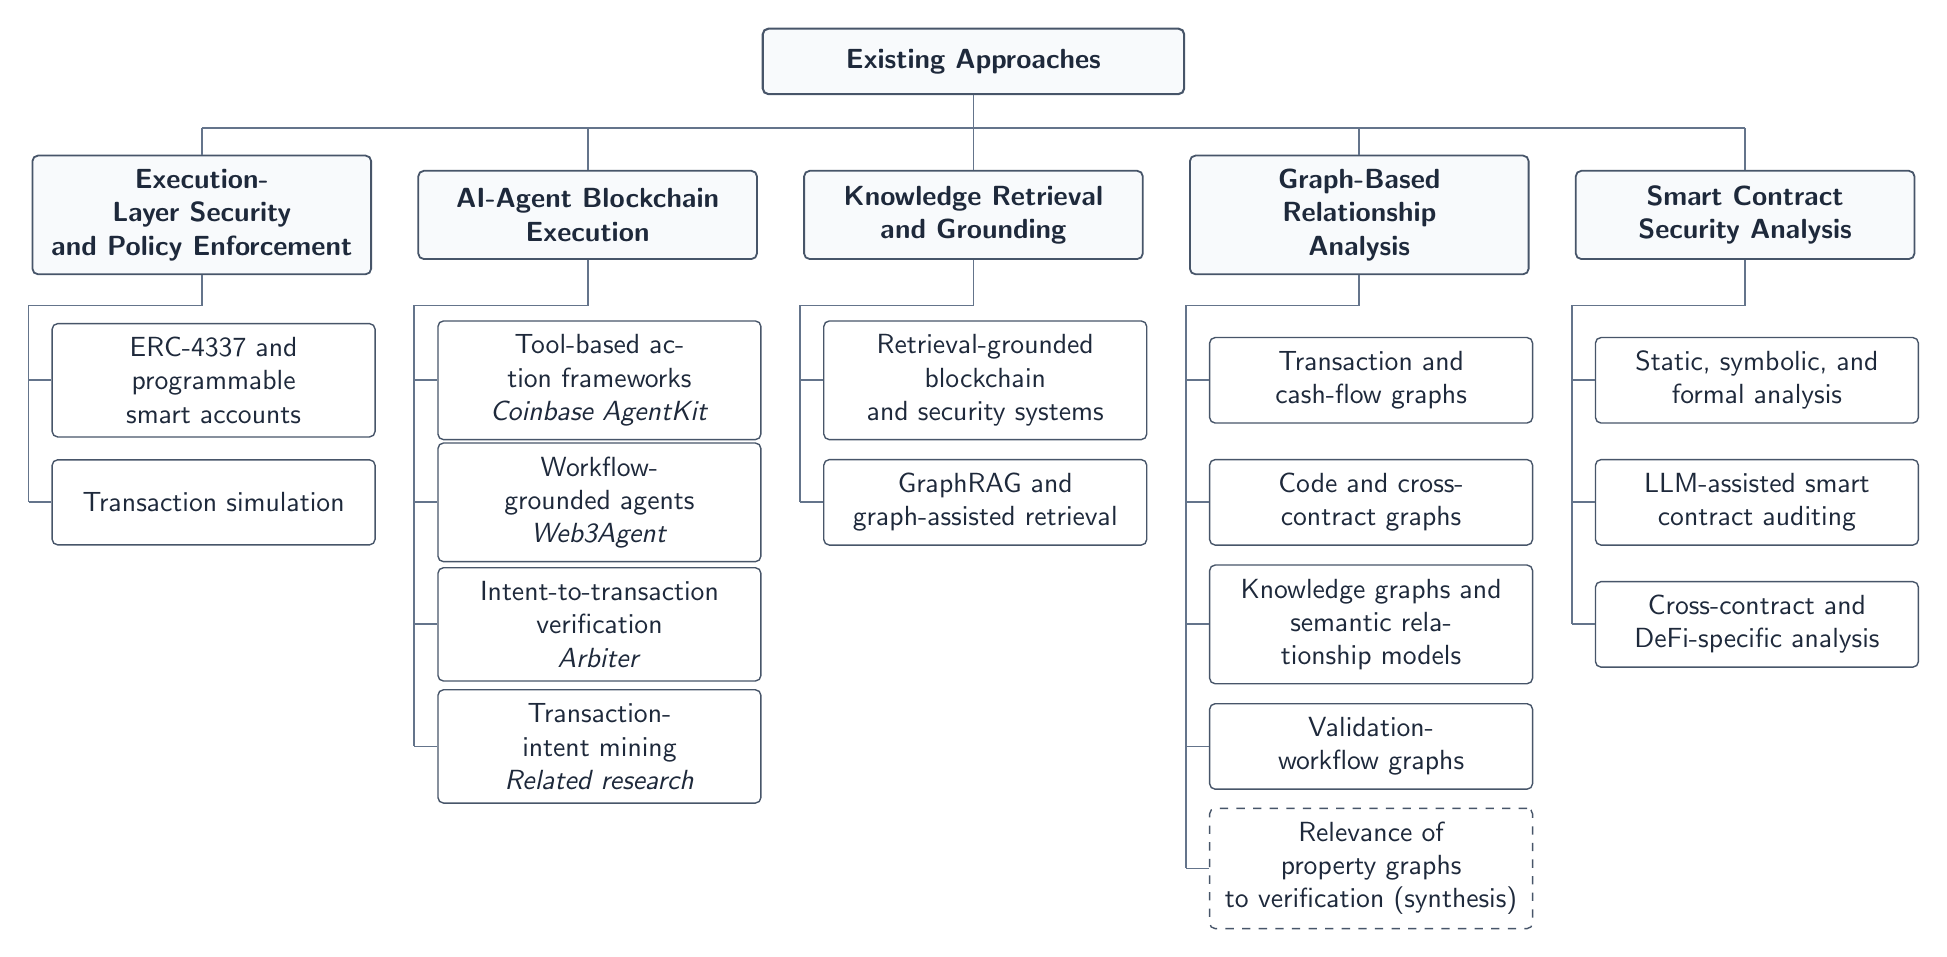
\begin{tikzpicture}[
    x=1cm, y=1cm,
    root/.style={
        draw=stepborder,
        fill=stepfill,
        rounded corners=2pt,
        line width=0.75pt,
        text=steptext,
        text width=5cm,
        minimum height=0.83cm,
        align=center,
        inner sep=5pt,
        font=\sffamily\bfseries
             \fontsize{10}{12}\selectfont
    },
    group/.style={
        draw=stepborder,
        fill=stepfill,
        rounded corners=2pt,
        line width=0.65pt,
        text=steptext,
        text width=3.95cm,
        minimum height=1.12cm,
        align=center,
        inner sep=5pt,
        font=\sffamily\bfseries
             \fontsize{10}{12}\selectfont
    },
    subgroup/.style={
        draw=stepborder,
        fill=white,
        rounded corners=2pt,
        line width=0.5pt,
        text=steptext,
        text width=3.75cm,
        minimum height=1.08cm,
        align=center,
        inner xsep=5pt,
        inner ysep=5pt,
        font=\sffamily
             \fontsize{10}{12}\selectfont
    },
    synthesis/.style={
        subgroup,
        dashed
    },
    link/.style={
        draw=arrowcol,
        line width=0.65pt
    }
]

% =====================================================
% LEVEL 1: ROOT
% =====================================================

\node[root] (root) at (0,0)
    {Existing Approaches};


% =====================================================
% LEVEL 2: FIVE APPROACH GROUPS
% =====================================================

\node[group] (g1) at (-9.8,-1.95)
    {Execution-Layer Security\\
     and Policy Enforcement};

\node[group] (g2) at (-4.9,-1.95)
    {AI-Agent Blockchain\\
     Execution};

\node[group] (g3) at (0,-1.95)
    {Knowledge Retrieval\\
     and Grounding};

\node[group] (g4) at (4.9,-1.95)
    {Graph-Based Relationship\\
     Analysis};

\node[group] (g5) at (9.8,-1.95)
    {Smart Contract\\
     Security Analysis};


% =====================================================
% ROOT-TO-GROUP BRANCHES
% =====================================================

\draw[link]
    (root.south) -- (0,-0.85);

\draw[link]
    (-9.8,-0.85) -- (9.8,-0.85);

\foreach \n in {1,2,3,4,5} {
    \draw[link]
        (g\n.north) --
        (g\n.north |- 0,-0.85);
}


% =====================================================
% LEVEL 3: GROUP 1
% Execution-Layer Security and Policy Enforcement
% =====================================================

\node[subgroup] (a1) at (-9.65,-4.05)
    {ERC-4337 and\\
     programmable smart accounts};

\node[subgroup] (a2) at (-9.65,-5.60)
    {Transaction simulation};


% =====================================================
% LEVEL 3: GROUP 2
% AI-Agent Blockchain Execution
% =====================================================

% Individual systems are representative examples.

\node[subgroup] (b1) at (-4.75,-4.05)
    {Tool-based action frameworks\\
     \textit{Coinbase AgentKit}};

\node[subgroup] (b2) at (-4.75,-5.60)
    {Workflow-grounded agents\\
     \textit{Web3Agent}};

\node[subgroup] (b3) at (-4.75,-7.15)
    {Intent-to-transaction verification\\
     \textit{Arbiter}};

\node[subgroup] (b4) at (-4.75,-8.70)
    {Transaction-intent mining\\
     \textit{Related research}};


% =====================================================
% LEVEL 3: GROUP 3
% Knowledge Retrieval and Grounding
% =====================================================

\node[subgroup] (c1) at (0.15,-4.05)
    {Retrieval-grounded blockchain\\
     and security systems};

\node[subgroup] (c2) at (0.15,-5.60)
    {GraphRAG and\\
     graph-assisted retrieval};


% =====================================================
% LEVEL 3: GROUP 4
% Graph-Based Relationship Analysis
% =====================================================

\node[subgroup] (d1) at (5.05,-4.05)
    {Transaction and\\
     cash-flow graphs};

\node[subgroup] (d2) at (5.05,-5.60)
    {Code and cross-contract graphs};

\node[subgroup] (d3) at (5.05,-7.15)
    {Knowledge graphs and\\
     semantic relationship models};

\node[subgroup] (d4) at (5.05,-8.70)
    {Validation-workflow graphs};

% The final box represents a synthesis, not
% a separate approach subgroup.

\node[synthesis] (d5) at (5.05,-10.25)
    {Relevance of property graphs\\
     to verification (synthesis)};


% =====================================================
% LEVEL 3: GROUP 5
% Smart Contract Security Analysis
% =====================================================

\node[subgroup] (e1) at (9.95,-4.05)
    {Static, symbolic, and\\
     formal analysis};

\node[subgroup] (e2) at (9.95,-5.60)
    {LLM-assisted smart\\
     contract auditing};

\node[subgroup] (e3) at (9.95,-7.15)
    {Cross-contract and\\
     DeFi-specific analysis};


% =====================================================
% CONNECTIONS: GROUP 1
% =====================================================

\draw[link]
    (g1.south) -- (-9.8,-3.10)
    -- (-12.0,-3.10)
    -- (-12.0,-5.60);

\draw[link]
    (-12.0,-4.05) -- (a1.west);

\draw[link]
    (-12.0,-5.60) -- (a2.west);


% =====================================================
% CONNECTIONS: GROUP 2
% =====================================================

\draw[link]
    (g2.south) -- (-4.9,-3.10)
    -- (-7.1,-3.10)
    -- (-7.1,-8.70);

\draw[link]
    (-7.1,-4.05) -- (b1.west);

\draw[link]
    (-7.1,-5.60) -- (b2.west);

\draw[link]
    (-7.1,-7.15) -- (b3.west);

\draw[link]
    (-7.1,-8.70) -- (b4.west);


% =====================================================
% CONNECTIONS: GROUP 3
% =====================================================

\draw[link]
    (g3.south) -- (0,-3.10)
    -- (-2.2,-3.10)
    -- (-2.2,-5.60);

\draw[link]
    (-2.2,-4.05) -- (c1.west);

\draw[link]
    (-2.2,-5.60) -- (c2.west);


% =====================================================
% CONNECTIONS: GROUP 4
% =====================================================

\draw[link]
    (g4.south) -- (4.9,-3.10)
    -- (2.7,-3.10)
    -- (2.7,-10.25);

\draw[link]
    (2.7,-4.05) -- (d1.west);

\draw[link]
    (2.7,-5.60) -- (d2.west);

\draw[link]
    (2.7,-7.15) -- (d3.west);

\draw[link]
    (2.7,-8.70) -- (d4.west);

\draw[link]
    (2.7,-10.25) -- (d5.west);


% =====================================================
% CONNECTIONS: GROUP 5
% =====================================================

\draw[link]
    (g5.south) -- (9.8,-3.10)
    -- (7.6,-3.10)
    -- (7.6,-7.15);

\draw[link]
    (7.6,-4.05) -- (e1.west);

\draw[link]
    (7.6,-5.60) -- (e2.west);

\draw[link]
    (7.6,-7.15) -- (e3.west);


\end{tikzpicture}%
}

\endgroup

\caption{Hierarchy of the five approach groups
and the subtopics reviewed.}

\label{fig:approach_hierarchy}

\end{figure}


% ============================================================
% 2.2.1
% ============================================================



\subsection{Execution-Layer Security and Policy Enforcement Approaches}
\label{subsec:execution_layer_security}

Execution-layer security approaches control whether a prepared
blockchain operation is authorised to proceed toward execution.
They typically operate after an action has been translated into
transaction parameters, a wallet request, or a smart-account
operation. Their primary concern is not the interpretation of
the user's original request, but whether the resulting operation
satisfies defined authorisation and execution conditions.

A central characteristic of this group is the enforcement of
restrictions on the authority available to an account or
automated agent. Such restrictions may concern the target
contract, callable function, recipient, token, amount, network,
or period during which an operation is permitted. Programmable
smart accounts support application-specific validation, while
modular account architectures allow additional authorisation
and execution mechanisms to be incorporated
\cite{buterinERC4337AccountAbstraction2021,
erc7579MinimalModularSmartAccounts2023}.
Permission mechanisms and transaction guards provide further
means of restricting automated operations
\cite{zeroDevPermissionsSessionKeys2026,
safeSmartAccountGuards2026}.

The result of an execution policy check is generally a decision
to permit or prevent an operation under the configured
conditions. Transaction simulation provides a related but
different form of pre-execution assessment. It examines the
expected behaviour of a prepared transaction and can reveal
execution failures or unexpected state changes without
submitting the transaction to the blockchain
\cite{tenderlyTransactionSimulation2026}. Simulation findings
can inform an execution decision, but they do not automatically
enforce one. These approaches are particularly relevant to AI-driven DeFi
because an automated agent may generate technically valid
operations that exceed its intended authority. Execution-layer
controls can restrict such operations independently of the
component that generated them. However, satisfying an execution
policy does not establish that the selected action correctly
represents the user's request. An agent may be authorised to
interact with an official protocol contract while selecting an
unintended function or asset. Execution control therefore
depends on separately defined rules or verification results
when intent correctness must also be established.

Two technical directions are considered within this group:
programmable smart accounts and policy controls, which restrict
execution authority, and transaction simulation, which examines
the expected effects of prepared operations.

\subsubsection{ERC-4337 and Programmable Smart Accounts}

Programmable smart accounts allow authorisation conditions to
be defined through account logic rather than relying only on
the signature-based authorisation of an Externally Owned
Account (EOA). This supports mechanisms such as delegated
permissions, restricted operations, and application-specific
validation rules. ERC-4337 introduces an account-abstraction architecture based
on \textit{UserOperations}, an EntryPoint contract, and
smart-account validation
\cite{buterinERC4337AccountAbstraction2021,
linMeasurementInvestigationERC43372024}.
A smart account validates a UserOperation according to its
implemented logic before execution. ERC-7579 extends the
design possibilities by specifying interfaces for modular
smart accounts and their validation and execution modules
\cite{erc7579MinimalModularSmartAccounts2023}.

Individual implementations demonstrate different policy
mechanisms. ZeroDev documents delegated permissions and
session keys that can restrict an automated process to
specified operations
\cite{zeroDevPermissionsSessionKeys2026}.
Safe Guards can inspect transaction parameters and prevent
execution when configured conditions are violated
\cite{safeSmartAccountGuards2026}.
Safe also describes smart-account applications involving
AI agents \cite{safeAIAgentsSmartAccounts2026}.

These mechanisms demonstrate how authorisation and execution
restrictions can be enforced, although the available controls
depend on the account implementation and its configuration.
Neither ERC-4337 nor programmable account logic inherently
determines whether a particular DeFi operation correctly
represents a natural-language intent. This requires additional
verification rules and reference information. Smart-account
mechanisms can enforce such a decision once it has been
established.

\subsubsection{Transaction Simulation}

Transaction simulation examines the expected execution of
a prepared blockchain transaction against a selected
blockchain state without committing its resulting changes.
It typically receives transaction parameters and calldata
and produces information about execution status, contract
calls, state changes, events, or asset movements. Tenderly provides a representative implementation, including
transaction traces, execution results, and state and asset
changes \cite{tenderlyTransactionSimulation2026}.
These results can help identify transactions that would
revert or behave unexpectedly before submission.

Simulation primarily answers the question:

\begin{quote}
``What is this prepared transaction expected to do?''
\end{quote}

The verification problem considered in this thesis asks:

\begin{quote}
``Does this execution information correctly represent the
user's requested action?''
\end{quote}

A transaction may simulate successfully while calling an
unintended but technically valid contract or function.
Simulation therefore provides useful behavioural evidence
but does not independently establish the correctness of
the intent-to-execution relationship. Preventing submission
based on simulation findings also requires an additional
enforcement mechanism.

\paragraph{Relationship to the requirements.}


Execution-layer security and policy enforcement approaches
primarily address R4 by restricting execution authority and
blocking operations that violate configured policies
\cite{buterinERC4337AccountAbstraction2021,
zeroDevPermissionsSessionKeys2026,
safeSmartAccountGuards2026}. Binding execution to verified
parameters depends on the implemented controls. Their contribution to R2 is limited to checking selected
transaction parameters, such as contracts, functions, or
recipients, without inherently validating the complete
intent-to-execution relationship. Similarly, R3 receives
limited support because authoritative knowledge acquisition
and maintenance are not intrinsic to these mechanisms.

These approaches can support R5 through identifiable policy
failures and simulation results, including transaction traces
\cite{safeSmartAccountGuards2026,
tenderlyTransactionSimulation2026}. However, the available
decision evidence depends on the implementation. They do
not inherently provide natural-language intent generation
under R1, while comparable verification-time measurements
for R6 are not established by the reviewed evidence.

\begin{table}[H]
\centering
\renewcommand{\arraystretch}{1.3}
\begin{tabular}{cccccc}
\hline
\textbf{R1} & \textbf{R2} & \textbf{R3} &
\textbf{R4} & \textbf{R5} & \textbf{R6} \\
\hline

$\circ\circ\circ$ &
$\star\circ\circ$ &
$\star\circ\circ$ &
$\star\star\star$ &
$\star\star\circ$ &
\textit{N/E} \\

\hline
\end{tabular}
\caption{Requirement coverage of execution-layer security
and policy enforcement approaches}
\label{tab:req_execution_layer}
\end{table}

% ============================================================
% 2.2.2
% ============================================================



\subsection{AI-Agent Blockchain Execution Approaches}
\label{subsec:ai_agent_blockchain_execution}

AI-agent blockchain execution approaches connect natural-language
interaction with blockchain operations. Their primary purpose is
to transform a user's request into a structured action that can
be processed by blockchain software. Depending on the approach,
the generated result may be a tool call, an execution plan,
transaction parameters, or a candidate blockchain operation.
Frameworks such as Coinbase AgentKit demonstrate how predefined
blockchain actions can be exposed to AI agents, while systems
such as Web3Agent incorporate workflow information into
blockchain interaction
\cite{coinbaseAgentKit2026,TODO_Web3Agent}.

A central characteristic of this group is the separation
between language-based action selection and the technical
operations performed by blockchain tools. Rather than allowing
an LLM to interact directly with arbitrary contracts, an
application may expose predefined actions with structured
input parameters. This constrains the available operations
and allows application code to handle transaction construction
and blockchain communication
\cite{coinbaseAgentKit2026}. Other approaches extend this
process by incorporating workflow reasoning or additional
checks before execution
\cite{TODO_Web3Agent,TODO_Arbiter2026}. The main contribution of these approaches is the conversion
of human-readable instructions into machine-readable blockchain
actions. This is particularly relevant to R1 because DeFi
operations require explicit parameters such as the action,
protocol, asset, amount, and recipient. However, producing
a structurally valid action does not establish that its
parameters correctly represent the user's intention.
An agent may select an available tool while providing an
incorrect network, contract, asset, or other execution
parameter. The distinction between action generation and
action verification is therefore important.

The reviewed literature covers several related technical
directions: tool-based blockchain action generation,
workflow-grounded agents, and intent-to-transaction
verification. Transaction-intent mining is also considered
as related research on the interpretation of blockchain
operations. These directions differ in their inputs,
mechanisms, and objectives, although they all contribute
to understanding the relationship between human intentions
and blockchain transactions.

\subsubsection{Tool-Based Blockchain Action Generation}

Tool-based approaches expose blockchain functionality through
predefined operations with structured parameters. The agent
selects an available operation and supplies the required
information, while application code performs the underlying
blockchain interaction. This reduces the need for the LLM
to generate unrestricted transaction logic. 

Coinbase AgentKit is a representative framework that provides
wallet providers and action providers for blockchain
interaction \cite{coinbaseAgentKit2026}. Action providers
define operations that an agent can invoke through structured
interfaces. The framework therefore supports the generation
of machine-readable blockchain actions and restricts the
operations exposed to the model. However, the availability of a structured action does not
independently establish that the selected protocol, contract,
function, and asset correspond to the user's request.
Verification may be implemented within an action provider
or through additional application components, but a
separate authoritative relationship-verification mechanism
is not inherent to the framework.

\subsubsection{Workflow-Grounded Blockchain Agents}

Workflow-grounded approaches extend action generation by
incorporating information about the steps, dependencies,
and conditions required to perform blockchain operations.
This allows the agent to consider whether a proposed
sequence of actions is feasible rather than selecting
individual tools without contextual information. 

Web3Agent represents this direction by combining
natural-language blockchain interaction with retrieved
workflow, API, and error-handling knowledge
\cite{TODO_Web3Agent}. Its workflow consistency and
contextual feasibility checks provide a form of
pre-execution assessment beyond structured action
generation alone. Nevertheless, workflow feasibility does not necessarily
establish that the underlying execution information is
authoritative or current. An operation may follow a
feasible workflow while relying on an outdated deployment,
incorrect network, or unsupported protocol resource.
Its contribution to authoritative verification therefore
depends on the reliability, applicability, and maintenance
of the information used.

\subsubsection{Intent-to-Transaction Verification}

Intent-to-transaction verification approaches examine whether
a proposed blockchain transaction is consistent with the
user's expressed objective. Unlike approaches primarily
concerned with generating actions, their main purpose is
to identify inconsistencies before execution.

Arbiter is a particularly relevant representative because
it compares a natural-language DeFi intent with a proposed
transaction \cite{TODO_Arbiter2026}. It combines technical
validation with LLM-supported semantic checks, including
canonical addresses, amounts, token decimals, slippage,
fees, deadlines, and potential parameter manipulation.
The system produces an auditable \textit{ACCEPT} or
\textit{REJECT} decision before execution. Arbiter also employs a Graph-of-Thoughts structure to
organise dependencies between validation operations.
This differs from a persistent property graph containing
protocol deployments, contracts, functions, assets,
pools, and reserves. Its graph structures the verification
procedure rather than maintaining the domain relationships
against which an execution path is checked. Arbiter demonstrates that pre-execution verification of
DeFi transactions against user intentions is already
being investigated. The relevant distinction for this
thesis is therefore not the existence of such verification,
but the representation and maintenance of authoritative
execution relationships and their use in deterministic
verification decisions.

\subsubsection{Transaction-Intent Mining}

Transaction-intent mining is a related research direction
that attempts to infer the purpose or semantic meaning
of blockchain transactions
\cite{TODO_TransactionIntentMining}. These approaches
typically examine observed transactions or historical
blockchain activity and may support classification,
monitoring, or forensic analysis. Their primary objective differs from pre-execution
verification. Transaction-intent mining generally asks
what an observed transaction was intended to accomplish,
whereas the problem considered in this thesis concerns
whether a proposed transaction should be accepted for
the current user request.

These approaches contribute to the understanding of
transaction semantics but do not inherently provide
authoritative pre-execution validation or execution
enforcement.

\paragraph{Relationship to the requirements.}

AI-agent blockchain execution approaches primarily support
R1 by transforming natural-language requests into structured
blockchain actions. Tool-based frameworks provide defined
action interfaces, while workflow-grounded agents incorporate
execution context \cite{coinbaseAgentKit2026,TODO_Web3Agent}.
However, detecting incomplete or ambiguous parameters is
not a general capability of the group. Individual approaches also contribute to R2. Web3Agent
examines workflow consistency and contextual feasibility,
while Arbiter performs pre-execution checks of transaction
consistency with user intent
\cite{TODO_Web3Agent,TODO_Arbiter2026}.
These mechanisms address aspects of intent validation but
do not, as a group, demonstrate systematic verification of
all action-specific execution relationships defined by R2.

Support for R3 depends on the authority, provenance, and
maintenance of external information. Similarly, R4 requires
enforcement mechanisms beyond producing a verification
decision. For R5, Arbiter demonstrates traceable validation
through identifiable checks and decision evidence
\cite{TODO_Arbiter2026}, although this capability is not
inherent to all AI-agent frameworks. For R6, the reviewed
results do not establish sufficiently comparable measurements
within the verification-time boundary defined in this thesis.

\begin{table}[H]
\centering
\renewcommand{\arraystretch}{1.3}
\begin{tabular}{cccccc}
\hline
\textbf{R1} & \textbf{R2} & \textbf{R3} &
\textbf{R4} & \textbf{R5} & \textbf{R6} \\
\hline

$\star\star\circ$ &
$\star\star\circ$ &
$\star\circ\circ$ &
$\star\circ\circ$ &
$\star\star\circ$ &
\textit{N/E} \\

\hline
\end{tabular}
\caption{Requirement coverage of AI-agent blockchain
execution approaches}
\label{tab:req_ai_agent}
\end{table}

% ============================================================
% 2.2.3
% ============================================================


\subsection{Knowledge Retrieval and Grounding Approaches}
\label{subsec:knowledge_retrieval_grounding}

Knowledge retrieval and grounding approaches obtain information
from external sources to support language models or other
processing components. Their main characteristic is the
separation of externally maintained knowledge from the
model or application that uses it. Retrieval-Augmented
Generation (RAG), for example, retrieves relevant information
from an external collection and incorporates it into the
generation process \cite{lewisRetrievalAugmentedGeneration2020}.
This allows information to be updated without retraining the
language model. The information processed by these approaches may include
documents, structured records, API responses, or connected
knowledge representations. Retrieval mechanisms identify
information relevant to a request and provide it as context
for subsequent interpretation, planning, or analysis.
Graph-assisted retrieval extends this process by considering
relationships between entities rather than relying only
on isolated documents
\cite{hanRetrievalAugmentedGenerationGraphs2025}.
The output is generally retrieved evidence or contextual
information, rather than an independently enforced
execution decision.

In blockchain applications, external knowledge may describe
protocol deployments, contract addresses, Application Binary
Interfaces (ABIs), supported assets, transaction workflows,
or security properties. Such information can help an agent
construct or examine blockchain operations. However,
retrieval relevance and information authority are different
properties. A retrieved document may be relevant to an
operation while describing another network, an outdated
deployment, or an unsupported protocol version.
Consequently, reliable verification requires additional
conditions concerning source authority, applicability,
provenance, and freshness. The literature considered in this group covers
retrieval-grounded blockchain and security systems,
together with GraphRAG and other graph-assisted retrieval
methods. Both directions use external information, but
they differ in how that information is organised and
selected for downstream processing.

\subsubsection{Retrieval-Grounded Blockchain and Security Systems}

Retrieval-grounded systems use external operational or
security knowledge to support blockchain-related tasks.
Web3Agent combines natural-language interaction with
workflow, API, and error-handling information to support
blockchain operations \cite{TODO_Web3Agent}. Retrieved
information contributes to planning and contextual
feasibility assessment. Retrieval is also used in smart-contract security analysis.
PropertyGPT, for example, retrieves existing security
properties to support the generation and verification
of properties for other contracts
\cite{TODO_PropertyGPT}. Other systems discussed in the
literature, including SmartProof, LLM-BSCVM, CyberTrust AI,
and Knowdit, investigate the use of external security
knowledge or contextual information in contract analysis
\cite{TODO_SmartProof,TODO_LLM_BSCVM,
TODO_CyberTrustAI,TODO_Knowdit}.

These examples demonstrate how externally stored knowledge
can support reasoning and analysis without being embedded
entirely in an LLM. However, their retrieval mechanisms do
not necessarily establish whether the information remains
authoritative for a particular DeFi deployment. Source
selection and knowledge maintenance must therefore be
considered separately from retrieval quality.

\subsubsection{GraphRAG and Graph-Assisted Retrieval}

GraphRAG incorporates graph-structured information into
retrieval and generation workflows. Instead of relying
exclusively on document similarity, these approaches may
retrieve connected entities, relationships, paths, or graph
summaries to provide additional context to a language model
\cite{hanRetrievalAugmentedGenerationGraphs2025}. Graph-assisted retrieval is particularly useful when
relevant information is distributed across several
connected entities. However, its effectiveness depends
on the graph construction method, retrieval strategy,
and evaluation setting
\cite{hanRAGGraphRAGSystematic2025,
hanRAGVsGraphRAG2026}.

The distinction from the verification problem considered
in this thesis concerns how the graph is used. GraphRAG
primarily retrieves relationship information to support
downstream reasoning or generation. A relationship-verification
mechanism instead evaluates defined conditions against
accepted reference information to determine whether a
specific execution relationship is supported. GraphRAG does not inherently guarantee that retrieved
relationships originate from authoritative sources, remain
current, or are used in a deterministic approval decision.
These properties require additional verification and
knowledge-management mechanisms.

\paragraph{Relationship to the requirements.}

Knowledge retrieval and grounding approaches contribute
primarily to R3 by supporting external knowledge access
and the extension of information sources
\cite{lewisRetrievalAugmentedGeneration2020,
hanRetrievalAugmentedGenerationGraphs2025}.
These capabilities are relevant to R3-C4, while source
identification and updating may support C2 and C3 in
individual implementations. However, retrieval alone
does not establish C1, which requires defined trusted
or authoritative sources. Since C1 is mandatory for a
rating above one star, the reviewed group is assessed
conservatively as providing limited R3 coverage.

These approaches can contribute to R2 by supplying
protocol or workflow information used in pre-execution
checks, as illustrated by retrieval-supported systems
such as Web3Agent \cite{TODO_Web3Agent}. Nevertheless,
retrieval does not inherently validate the complete
action-specific execution relationships required by R2.
The group does not independently provide structured
intent generation under R1, execution enforcement under
R4, or a traceable verification decision under R5.
For R6, comparable verification-time measurements are
not established by the reviewed evidence.

\begin{table}[H]
\centering
\renewcommand{\arraystretch}{1.3}
\begin{tabular}{cccccc}
\hline
\textbf{R1} & \textbf{R2} & \textbf{R3} &
\textbf{R4} & \textbf{R5} & \textbf{R6} \\
\hline

$\circ\circ\circ$ &
$\star\circ\circ$ &
$\star\circ\circ$ &
$\circ\circ\circ$ &
$\circ\circ\circ$ &
\textit{N/E} \\

\hline
\end{tabular}
\caption{Requirement coverage of knowledge retrieval
and grounding approaches}
\label{tab:req_knowledge_retrieval}
\end{table}



% ============================================================
% 2.2.4
% ============================================================


\subsection{Graph-Based Relationship Analysis Approaches}
\label{subsec:graph_structured_approaches}

Graph-based relationship analysis approaches represent
information through entities and explicit connections
between them. Their central characteristic is the
ability to examine relationships rather than treating
each entity independently. Depending on the application,
graphs may represent transaction flows, program
dependencies, domain knowledge, or the dependencies
between validation operations
\cite{hoganKnowledgeGraphs2021,
anglesPropertyGraphModel2018}. The mechanisms used in this group include graph construction,
traversal, pattern matching, and structural analysis. Their
inputs may consist of transaction histories, contract code,
structured records, or domain-specific information. The
result can be a classification, an identified dependency,
a matched relationship pattern, or evidence of a violated
constraint. Graph query languages such as Cypher provide
a means of examining connected structures through explicit
patterns \cite{francisCypher2018}.

However, the presence of a graph does not establish that
its information is trustworthy or that its conclusions
are suitable for execution decisions. Graph correctness
depends on the represented entities and relationships,
their sources, and the rules used to interpret them.
Provenance models and graph validation mechanisms provide
ways to describe information origins and structural
constraints, but they do not independently guarantee
source authority or freshness
\cite{w3cPROVO2013,w3cSHACL2017}. The reviewed literature covers four distinct directions:
transaction and cash-flow graphs, code and cross-contract
graphs, knowledge graphs and semantic relationship models,
and validation-workflow graphs. Their common characteristic
is the analysis of connected information, while the meaning
of the graph and its analytical objective differ.

\subsubsection{Transaction and Cash-Flow Graphs}

Transaction and cash-flow graphs represent relationships
between blockchain accounts, contracts, transfers, and
asset movements. They are commonly used to examine
transaction behaviour, temporal patterns, and the flow
of assets between entities.

Graph-based fraud detection approaches, DeFiGuard, and
RugScreener illustrate this direction by analysing
transaction or temporal relationships to identify
suspicious behaviour and potential security risks
\cite{TODO_DeFiGraphTransformerFraud,
TODO_DeFiGuard,TODO_RugScreener}. These approaches are valuable for monitoring and
behavioural analysis. However, identifying suspicious
transaction patterns differs from establishing whether
a selected protocol, contract, function, and asset
form the correct execution relationship for a user's
request. Their findings may provide additional risk
information but do not independently satisfy the
action-specific validation required by R2.

\subsubsection{Code and Cross-Contract Graphs}

Code-oriented graphs represent relationships within
or between smart contracts, including function calls,
control flow, data dependencies, and contract
interactions. Their purpose is to expose program
structures that may be difficult to analyse through
individual code elements.

Approaches such as CHAINTRIX, DeFiTail, DeFiTainter,
and CoTA investigate contract interactions and
dependencies to identify vulnerabilities or unsafe
behaviour
\cite{TODO_CHAINTRIX,TODO_DeFiTail,
TODO_DeFiTainter,TODO_CoTA}. These analyses can contribute evidence about contract
behaviour and potential security weaknesses. However,
a function or interaction that is not identified as
vulnerable is not necessarily the correct one for
a particular natural-language DeFi request. Code
relationship analysis therefore serves a different
purpose from intent-to-execution relationship
verification.

\subsubsection{Knowledge Graphs and Semantic Relationship Models}

Knowledge graphs represent domain-specific entities and
their semantic relationships. Unlike graphs derived
primarily from transaction activity or program code,
their structure is intended to describe knowledge about
a particular domain. Hogan et al.\ discuss knowledge
graph models, query languages, and related validation
mechanisms \cite{hoganKnowledgeGraphs2021}.
Property graphs associate labels and properties with
nodes and relationships, allowing contextual information
to accompany the represented connections
\cite{anglesPropertyGraphModel2018}. These representations can support explicit queries over
connected entities. Cypher, for example, provides
pattern-matching operations for property graphs
\cite{francisCypher2018}. In a DeFi verification context,
such patterns could represent associations between
protocol deployments, supported actions, contracts,
functions, assets, pools, and reserves.

Research on the integration of language models and
knowledge graphs also distinguishes graph-supported
reasoning from model-assisted graph construction
\cite{panUnifyingLargeLanguage2023}.
Blockchain-related applications such as Knowdit and
cryptoasset entity-linking approaches demonstrate uses
of structured knowledge for security analysis and
attribution
\cite{TODO_Knowdit,TODO_CryptoassetEntityLinking}. The relevance to this thesis lies in representing
execution-related information as connected entities
rather than independent records. Nevertheless, a
successful graph query establishes consistency with
stored relationships. It does not independently prove
that those relationships are authoritative, complete,
or current.

\subsubsection{Validation-Workflow Graphs}

Validation-workflow graphs represent the dependencies
between checks rather than the domain information
being checked. They can organise the order of validation
operations, express dependencies between conditions,
and combine individual findings into a decision.

Arbiter provides a relevant example through its
Graph-of-Thoughts-based validation structure
\cite{TODO_Arbiter2026}. Its approach combines
technical and semantic checks to examine the
consistency between a proposed DeFi transaction
and the user's intent. The important distinction concerns what the graph
represents. Arbiter's graph organises the validation
procedure, whereas a domain knowledge graph can
represent persistent information about protocol
deployments and their execution relationships.
These representations may complement one another,
but their purposes are not equivalent.


\subsubsection{Relevance of Property Graphs to Verification}

Representing relationships and validating graph
information are separate concerns. PG-Schema
introduces type definitions and constraints for
property graphs \cite{anglesPGSchema2023}.
For RDF graphs, SHACL provides a means of defining
structural constraints and producing validation
reports \cite{w3cSHACL2017}. Corman et al.\
also investigate the semantics of recursive shape
constraints \cite{cormanRecursiveSHACL2018}. These mechanisms demonstrate how graph data can
be checked against defined structural requirements.
However, schema conformance does not establish
whether an address or relationship is authoritative
for a particular blockchain deployment.

Provenance and completeness are further considerations.
PROV-O provides a vocabulary for representing the
origins and derivation of information
\cite{w3cPROVO2013}. Darari et al.\ investigate
completeness statements for RDF data sources and
their use in reasoning about query answers
\cite{darariCompletenessRDF2018}. This distinction is particularly relevant when
verification depends on the absence of a relationship.
A missing graph connection may indicate an unsupported
operation, but it may also result from incomplete
knowledge. Treating absence as evidence against an
operation requires sufficient knowledge coverage
for the relevant verification context.

Property graphs therefore provide a suitable
representation for examining connected execution
information through action-specific queries.
Their use as a verification mechanism requires
additional decisions concerning source authority,
knowledge maintenance, completeness, and the
conditions under which query results lead to
approval or rejection.

\paragraph{Relationship to the requirements.}

Graph-based relationship analysis approaches provide
limited support for R2 through explicit representation
and examination of connected entities
\cite{anglesPropertyGraphModel2018,francisCypher2018}.
Graph patterns can express conditions relevant to
R2-C1 through R2-C3 when the required domain
relationships are modelled. However, the reviewed
graph mechanisms do not inherently implement all
these checks for DeFi operations or ensure their
application before execution under C4. For R3, graph models can support extensible
relationships and contextual metadata, while
provenance mechanisms can identify information origins
\cite{hoganKnowledgeGraphs2021,w3cPROVO2013}.
These capabilities relate to R3-C2 and R3-C4.
However, neither authoritative source acquisition
under C1 nor reliable invalidation of outdated
information under C3 follows from graph representation
alone. The group therefore receives limited R3
coverage rather than a higher rating.

Graph queries and constraint-validation mechanisms
can also contribute to R5 by exposing matched
relationships or identifiable violations
\cite{francisCypher2018,w3cSHACL2017}.
This supports parts of R5-C2 and R5-C3, but does not
inherently provide a complete intent-verification
decision satisfying R5-C1 and R5-C4. Graph representation does not independently perform
natural-language intent generation under R1 or enforce
wallet execution restrictions under R4. For R6,
the reviewed literature does not establish comparable
measurements for the pre-execution verification
boundary defined in this thesis.

\begin{table}[H]
\centering
\renewcommand{\arraystretch}{1.3}
\begin{tabular}{cccccc}
\hline
\textbf{R1} & \textbf{R2} & \textbf{R3} &
\textbf{R4} & \textbf{R5} & \textbf{R6} \\
\hline

$\circ\circ\circ$ &
$\star\circ\circ$ &
$\star\circ\circ$ &
$\circ\circ\circ$ &
$\star\circ\circ$ &
\textit{N/E} \\

\hline
\end{tabular}
\caption{Requirement coverage of graph-based
relationship analysis approaches}
\label{tab:req_graph_structured}
\end{table}


% ============================================================
% 2.2.5
% ============================================================

\subsection{Smart Contract Security Analysis Approaches}
\label{subsec:smart_contract_security}

Smart contract security analysis approaches examine the
implementation and behaviour of blockchain programs to
identify vulnerabilities, incorrect behaviour, and violations
of specified properties. Their inputs may include source code,
bytecode, execution traces, program dependencies, and formal
specifications. The main objective is to determine whether
a contract or interaction exhibits security weaknesses,
rather than whether it represents a particular user's
intended transaction. 

The group includes static analysis, symbolic execution,
formal verification, and LLM-assisted analysis. These
mechanisms differ in how they examine contract behaviour.
Static techniques inspect program structures and dependencies,
while symbolic and formal methods reason about possible
execution paths or specified properties. LLM-assisted systems
incorporate language-model reasoning into security analysis,
often alongside more structured validation mechanisms
\cite{sunGPTScanDetectingLogic2023,
weiLLMSmartAuditAdvanced2024,
TODO_PropertyGPT}. The results of these approaches commonly include vulnerability
findings, affected code locations, execution traces, violated
properties, or verification outcomes. Such evidence can support
the assessment of contract security, although the absence of
detected vulnerabilities does not establish that a contract is
free of all weaknesses. DeFi applications introduce additional
complexity because relevant behaviour may involve interactions
between several contracts rather than a single program
\cite{TODO_DeFiTail,TODO_DeFiTainter,
TODO_CHAINTRIX}. 

Three technical directions are considered: static, symbolic,
and formal analysis; LLM-assisted smart contract auditing;
and cross-contract and DeFi-specific analysis. They differ
in their analysis mechanisms but share the objective of
examining contract behaviour for security problems.

\subsubsection{Static, Symbolic, and Formal Analysis}

Static and symbolic approaches examine possible contract
behaviour through program analysis, execution paths,
or logical constraints. Formal verification further
examines whether specified properties hold under
defined assumptions.

Systems such as SymGPT, FairChecker, and OVer investigate
symbolic reasoning or formalised constraints for identifying
contract-level problems
\cite{TODO_SymGPT,TODO_FairChecker,TODO_OVer}.
PropertyGPT and SmartProof additionally investigate
the generation, retrieval, or verification of contract
security properties
\cite{TODO_PropertyGPT,TODO_SmartProof}. These approaches can provide structured evidence about
contract behaviour. However, satisfying a security
property does not establish that the analysed contract
or function is appropriate for a specific natural-language
DeFi request. Their main contribution is therefore
contract-level assurance rather than intent-to-execution
relationship validation.

\subsubsection{LLM-Assisted Smart Contract Auditing}

LLM-assisted auditing combines language-model capabilities
with security analysis to identify potential vulnerabilities
or violations of expected behaviour. GPTScan combines LLM-supported identification of logic
vulnerabilities with program analysis
\cite{sunGPTScanDetectingLogic2023}.
LLM-SmartAudit uses specialised LLM agents for
smart-contract security analysis
\cite{weiLLMSmartAuditAdvanced2024}.
LogicScan examines business-logic vulnerabilities using
structured specifications and contrastive analysis
\cite{gaoLogicScanLLMDriven2026}.
Related systems, including LLM-BSCVM and CyberTrust AI,
investigate LLM-supported or knowledge-grounded contract
analysis
\cite{TODO_LLM_BSCVM,TODO_CyberTrustAI}.

These systems illustrate how probabilistic language-model
reasoning can support security analysis alongside more
structured methods. Nevertheless, identifying a potential
vulnerability remains different from determining whether
a proposed blockchain operation correctly represents the
user's intended action.

\subsubsection{Cross-Contract and DeFi-Specific Analysis}

Cross-contract analysis considers dependencies and
interactions between several contracts. This is relevant
to DeFi applications, where the behaviour of an operation
may depend on multiple interacting components. DeFiTail, DeFiTainter, and CHAINTRIX investigate
cross-contract interactions, dependencies, or information
flows to identify potentially unsafe behaviour
\cite{TODO_DeFiTail,TODO_DeFiTainter,
TODO_CHAINTRIX}.

Such analysis may provide evidence that a contract,
function, or interaction should not be trusted. However,
a contract that passes the relevant security analysis
is not necessarily the correct contract for a requested
DeFi action. Contract security analysis and
intent-to-execution relationship verification therefore
address complementary concerns.

\paragraph{Relationship to the requirements.}

Smart contract security analysis approaches contribute
primarily to the assessment of contract behaviour.
Their relevance to R3 lies in producing identifiable
security findings associated with analysed contracts
or functions, which may provide supporting evidence
for R3-C2
\cite{sunGPTScanDetectingLogic2023,
TODO_PropertyGPT}. However, these findings do not
inherently establish authoritative verification sources
under C1 or provide the knowledge-maintenance mechanisms
required by C3 and C4. R3 coverage is therefore limited. The group also provides limited support for R5 through
identified vulnerabilities, affected code locations,
and violated security properties
\cite{sunGPTScanDetectingLogic2023,
gaoLogicScanLLMDriven2026}. These results may support
R5-C2 and R5-C3, but they do not constitute a complete
intent-verification decision.

The reviewed mechanisms do not independently satisfy
the action-specific checks required by R2. In particular,
analysing contract behaviour does not establish that
the selected deployment, function, and asset correspond
to the user's requested operation. Accordingly, the
group is not credited with direct R2 coverage under
the defined assessment criteria. These approaches do not inherently provide natural-language
intent generation under R1 or wallet-level execution
enforcement under R4. For R6, the reviewed measurements
are not sufficiently comparable with the verification-time
boundary defined in this thesis.

\begin{table}[H]
\centering
\renewcommand{\arraystretch}{1.3}
\begin{tabular}{cccccc}
\hline
\textbf{R1} & \textbf{R2} & \textbf{R3} &
\textbf{R4} & \textbf{R5} & \textbf{R6} \\
\hline

$\circ\circ\circ$ &
$\circ\circ\circ$ &
$\star\circ\circ$ &
$\circ\circ\circ$ &
$\star\circ\circ$ &
\textit{N/E} \\

\hline
\end{tabular}
\caption{Requirement coverage of smart contract
security analysis approaches}
\label{tab:req_smart_contract_security}
\end{table}


%   2.3   Comparison


\section{Comparison of Approaches}
\label{sec:sota_comparison}

The five approach groups reviewed in
Section~\ref{sec:sota_approaches} address different aspects
of secure AI-driven DeFi execution. Table~\ref{tab:requirements_approach_comparison}
summarises their coverage of the six requirements defined
in Section~\ref{sec:requirements_analysis}. The ratings
follow the requirement-specific assessment criteria and
the evidence discussed for each group. They represent
a synthesis of the reviewed mechanisms rather than
capabilities shared by every system within a group.
The supporting criterion-level assessments and their
evidence are provided in
Appendix~\ref{app:requirement_assessment}.

\begin{table}[H]
\centering
\renewcommand{\arraystretch}{1.4}
\resizebox{\textwidth}{!}{%
\begin{tabular}{lcccccc}
\hline
\textbf{Approach Group}
& \textbf{R1}
& \textbf{R2}
& \textbf{R3}
& \textbf{R4}
& \textbf{R5}
& \textbf{R6} \\
\hline

Execution-Layer Security and Policy Enforcement
& $\circ\circ\circ$
& $\star\circ\circ$
& $\star\circ\circ$
& $\star\star\star$
& $\star\star\circ$
& \textit{N/E} \\

AI-Agent Blockchain Execution
& $\star\star\circ$
& $\star\star\circ$
& $\star\circ\circ$
& $\star\circ\circ$
& $\star\star\circ$
& \textit{N/E} \\

Knowledge Retrieval and Grounding
& $\circ\circ\circ$
& $\star\circ\circ$
& $\star\circ\circ$
& $\circ\circ\circ$
& $\circ\circ\circ$
& \textit{N/E} \\

Graph-Based Relationship Analysis
& $\circ\circ\circ$
& $\star\circ\circ$
& $\star\circ\circ$
& $\circ\circ\circ$
& $\star\circ\circ$
& \textit{N/E} \\

Smart Contract Security Analysis
& $\circ\circ\circ$
& $\circ\circ\circ$
& $\star\circ\circ$
& $\circ\circ\circ$
& $\star\circ\circ$
& \textit{N/E} \\

\hline
\end{tabular}%
}
\caption{Requirement coverage of the reviewed approach groups
according to the assessment criteria defined in
Section~\ref{sec:requirements_analysis}.}
\label{tab:requirements_approach_comparison}
\end{table}



The comparison shows that AI-agent approaches contribute
most directly to structured intent generation (R1),
while individual systems also demonstrate pre-execution
validation capabilities relevant to R2. Execution-layer
security provides the strongest mechanisms for enforcing
execution restrictions (R4). Knowledge retrieval and
graph-based analysis offer complementary means of obtaining
and representing verification information. However, neither
inherently establishes the source authority required by
R3-C1. Their limited R3 ratings reflect this restriction
rather than a judgement that one representation is
inherently superior.

Several groups also contribute to traceability (R5),
although the evidence they produce serves different
purposes. Contract security findings, graph relationships,
and policy failures do not necessarily explain the same
verification decision. For R6, the reviewed measurements
are not sufficiently comparable with the defined
pre-execution verification boundary, and no rating
is assigned.

Overall, the comparison indicates that the requirements
are addressed through complementary mechanisms rather
than a single approach group. The suitability of a
mechanism therefore depends on its intended role within
the verification process. The possible technical directions arising from this
comparison and their remaining limitations are discussed
in the following sections.


% alternative appraoches

\section{Possible Approaches to Pre-Execution Verification}
\label{sec:sota_alternative_approaches}

The comparison in Section~\ref{sec:sota_comparison} indicates
that the requirements for pre-execution DeFi verification
could be addressed through different technical approaches
or combinations of mechanisms. An important design choice
concerns how execution relationships are represented,
validated, and connected to the remaining transaction
workflow.

One possibility is rule-based verification using predefined
deployment registries and application-level checks.
Information about supported protocols, contracts, functions,
and assets could be maintained in a registry and compared
against a proposed operation. This approach provides explicit
validation conditions and is suitable for a clearly defined
set of operations. However, changes to protocol deployments
or supported resources require the registry and corresponding
rules to be maintained consistently. 

A relational database offers another possibility. Networks,
protocol deployments, contracts, functions, and assets can
be represented through related tables. Queries involving
joins and constraints can then examine whether the selected
entities form an accepted execution relationship. This
provides a structured alternative to graph-based verification,
although the required relationships and validation conditions
must still be defined explicitly.

Graph-based approaches offer a different representation
of connected execution information. RDF supports semantic
relationships, while SHACL provides mechanisms for expressing
and validating graph constraints \cite{w3cSHACL2017}.
Property graphs represent entities and their relationships
with associated properties \cite{anglesPropertyGraphModel2018}.
Cypher allows connected patterns to be queried explicitly
\cite{francisCypher2018}, while PG-Schema provides structural
definitions and constraints \cite{anglesPGSchema2023}.
These mechanisms are suitable for expressing action-specific
execution relationships, although their correctness still
depends on the authority and maintenance of the underlying
information.

Beyond the representation of verification knowledge, the
reviewed approaches suggest possible combinations across
different stages of the transaction workflow. AI-agent
frameworks could generate structured intents, while external
information sources supply protocol and deployment knowledge.
Rule-based or relationship-based verification could then
examine the proposed execution information before passing
an accepted operation to a controlled execution mechanism.
Programmable smart accounts and transaction policies provide
possible means of enforcing the resulting decision
\cite{coinbaseAgentKit2026,
buterinERC4337AccountAbstraction2021,
safeSmartAccountGuards2026}. Transaction simulation and
smart-contract security analysis could provide additional
evidence about execution behaviour and contract security.

These directions are not mutually exclusive, and none
requires a particular database technology. Their suitability
depends on the complexity of the relationships being verified,
the reliability and maintenance of reference information,
and the ability to enforce verification decisions. The
remaining limitations relevant to the problem considered
in this thesis are discussed in the following section.



\section{Limitations of Existing Approaches}
\label{sec:sota_limitations}

The reviewed approaches provide relevant capabilities for
AI-driven DeFi execution, but the available evidence does
not establish a single integrated mechanism satisfying all
the requirements defined in
Section~\ref{sec:requirements_analysis}.

A central limitation concerns the connection between
structured intent generation and execution-specific
verification. AI-agent approaches can construct blockchain
operations, and systems such as Web3Agent and Arbiter
demonstrate forms of pre-execution validation
\cite{TODO_Web3Agent,TODO_Arbiter2026}.
However, these capabilities do not necessarily establish
that all required protocol, deployment, contract, function,
and asset relationships are verified against maintained
authoritative information. Verification knowledge introduces a further challenge.
Retrieval systems and graph-based representations can make
external information accessible and examine its relationships,
but the reliability of a decision also depends on source
authority, freshness, and knowledge completeness. In
particular, a missing relationship cannot automatically
be interpreted as evidence that an operation is invalid
when the available knowledge may be incomplete.

Finally, producing a verification decision is different
from enforcing it. Execution controls must prevent
unapproved operations from proceeding and ensure that
approved execution remains bound to the verified parameters.
Traceable decisions and bounded verification time introduce
additional requirements that are not consistently
demonstrated across the reviewed approaches.

The remaining research problem is therefore not the absence
of individual verification or security mechanisms, but
their integration into a pre-execution process that connects
structured user intents, authoritative execution relationships,
and controlled transaction execution. The following chapter
develops a graph-based verification concept for this purpose
and explains the selection and integration of its components.



\section{Summary}
\label{sec:sota_summary}

This chapter defined six requirements for secure AI-driven
DeFi execution and reviewed five groups of existing
approaches. The literature review examined their technical
characteristics, representative systems, and contributions
to the requirements. The comparison showed that AI-agent
approaches support structured action generation, execution-layer
mechanisms provide transaction restrictions, and retrieval
and graph-based approaches offer complementary means of
managing and examining information. Smart contract security
analysis provides additional evidence concerning contract
behaviour and vulnerabilities.

The review also considered possible directions for
pre-execution verification, including rule-based registries,
relational databases, graph-based representations, and
combinations of mechanisms from different approach groups.
These alternatives demonstrate that relationship verification
is not restricted to a particular technology. However,
the reviewed evidence does not establish a single integrated
approach that satisfies all the defined requirements.
In particular, authoritative knowledge maintenance,
action-specific relationship validation, and enforcement
of verification decisions require further integration.

The findings provide the basis for the concept developed
in the following chapter. It investigates how structured
DeFi intents can be verified against maintained authoritative
execution relationships using a property graph and how
the resulting decisions can be incorporated into a
controlled pre-execution workflow.
